% !TEX root = ../main.tex
\subsubsection{Geometry Effect}
\label{sssec::geometry_effect}
    % The effect has already been presented and discussed before, so we're brief.
    This problem is already discussed in detail in section \ref{sssec::geometry_effect}.
    As a quick reminder, FMT sits at $z \approx 26$ cm, and it naturally performs poorly for targets to close to it.
    We can measure the strength of this effect by applying the geometry cut given by equation \eqref{eq::fmt_geometry_cut} to both DC and FMT tracks.
    Figure \ref{fig::vz_012016_geomcut} the effect of the cut when applied on figure \ref{fig::vz_012016}.
    Its effect on a $v_z$ vs $\theta$ plot can be seen on figure \ref{fig::vz_vs_theta}.

    Based on this cut and the FMT $z$ position, subsequent plots will be constrained to the range $-30 \text{[cm]} < v_z < 20 \text{[cm]}$.

    \begin{figure}[h!]
        \centering\frame{
        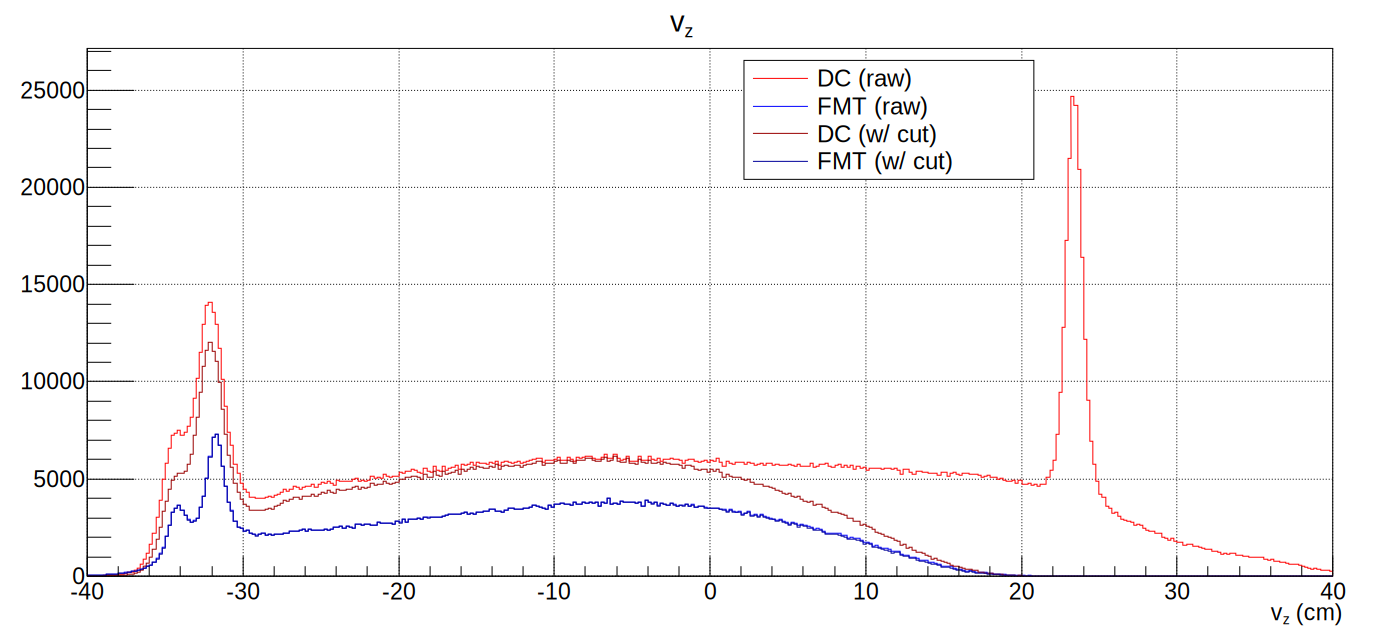
\includegraphics[width=\textwidth]{12vz_012016_geomcut.pdf}}
        \caption[$v_z$ for DC and FMT, w/ and w/out the geometry cut, run 12016]{$v_z$ for DC without the geometry cut (in red), with it (in dark red), for FMT without it (in blue), and with it (in dark blue). Spring 2020 data, run 12016. The effect is very clear on DC tracks, yet it almost doesn't affect FMT tracks.}
        \label{fig::vz_012016_geomcut}
    \end{figure}
